\documentclass{kthreport}

\usepackage{hhline}
\usepackage[parfill]{parskip}
\usepackage{subcaption}
\usepackage{placeins}
\usepackage{todonotes}
\usepackage{graphicx,wrapfig,lipsum}

\pagestyle{plain}
\pagenumbering{arabic}

\title{Classification of ImageNet with Convolutional Neural Networks}
\subtitle{A study in techniques to improve CNN's}
\author{W. Skagerström, T. Price, N. Lindqvist}
\diarienr{Deepl-18 Project}

\begin{document}
\maketitle
\newpage
\begin{abstract}

\noindent This report is our final piece of work in the course DD2424, Deep Learning in Data Science. The overarching purpose is to investigate convolutional neural networks (CNNs) while applying knowledge and techniques which we've acquired during the course.\\

\noindent To thoroughly investigate the topic, a CNN will be constructed. The architecture will be based on research of previous state of the art implementations on the topic. The network will be optimized iteratively by more sophisticated initialization, changing activation functions and additional optimization and regularization such as dropout and batch normalization. The effect of each modification will be documented and analyzed. The results are then discussed on their own and in context of other ImageNet classifiers.\\

\noindent We implemented a VGGNet which initially suffered immensely by overfitting. By tinkering with parameters of dropout, L2 regularization and batch normalization we countered the effect to some extent but not fully. We achieved a maximum accuracy of 29\%. All in all we learned a lot and conclude that optimization of CNNs is a difficult craft.

\end{abstract}
\newpage

\tableofcontents
\newpage

\section{Introduction}
Image classification is one of the main branches within Computer Vision. The task can be summarized as extracting features from a picture, which takes the shape of a pixel matrix containing either 1 or 3 channels (for gray-scale or RGB, respectively). Back in 2012, Convolutional Neural Networks (CNNs) began replacing the previously manually written algorithms for feature detection, and continue to hold the title as a state of the art method for image classification. The reason for the resurgence of CNNs was partly due to the winning entry of the AlexNet in the 2012 ImageNet competition \cite{krizhevsky2012imagenet}. Convolutional Neural Networks have existed for almost 20 years, but was previously limited by the availability of data and computer hardware. However, due to the great advancement of modern computers the ability to train increasingly deep and complex types of neural networks have been enabled.

In 2014, another progressive leap in the development of image classification occurred with the introduction of VGGNet and GoogleNet \cite{simonyan2014very}, \cite{szegedy2016rethinking}.  Due to the possibility of creating CNNs of varying architecture and size, a modern industry standard for evaluating the performance of a network is by benchmarking it through the ImageNet dataset \cite{russakovsky2015imagenet}.


\section{Previous work}
\label{sec:PreviousWork}
Among the many entries to the ImageNet classification challenge, deep convolution network architectures such AlexNet, VGGNet and GoogleNet have proven themselves to be highly effective and has created a renewed interest in the development and optimization of such architectures. However, these different types of network comes with some individual strengths and weaknesses.

\subsection{AlexNet}
AlexNet is the network architecture that renewed the industry interest in Convolutional Neural networks. AlexNet consists of a total of 8 layers, which are 5 convolutional layers which are stacked on each other, followed by three fully connected layers. The network features two sets of of batch normalization, which are applied following each of the first two convolution layers, and a dropout occurs after each of the last two fully connected layers. Compared to the other networks mentioned here, it performs slightly worse in terms of accuracy as seen in figure \ref{wrap-fig:graph_cnns}.

\clearpage
\subsection{GoogLeNet}
%------------------------------------------
\begin{wrapfigure}{r}{0.6\linewidth}
  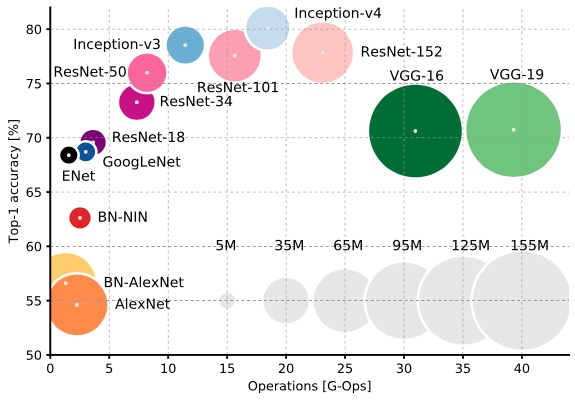
\includegraphics[width=\linewidth]{../images/graph_cnns.jpg}
  \caption[]
  {\small Comparision of performance, amount of parameters and number of operations between different CNNs.}
  \label{wrap-fig:graph_cnns}
\end{wrapfigure}
%------------------------------------------
GoogLeNet uses what is called a inception module, which works by calculating several different convolutions of different dimension within the same module combining them before propagating them to the next layer of the network\cite{szegedy2016rethinking}. This causes GoogLeNet to be much more space efficient due to the less  amount of parameters. This is only further amplified by the usage of average pooling instead of fully connected layers, which further reduces the dimensionality of the total number of network parameters, see figure \ref{wrap-fig:graph_cnns}. \\

\subsection{ResNet}
ResNet was added to the different architectures of networks for image classification in 2015 and won the 1st place on the ILSVRC 2015 classification task. As deeper networks are more difficult to train a residual learning framework eases the training for deep networks by adding a shortcut between layers. The shortcut decreases the complexity of the networks and witch allows more layers \cite{HeZRS15}.

\subsection{VGGNet}
VGGNet was introduced in 2014 and one of its most common characteristics is the simplicity of the network, while still achieving good performance on complicated classification tasks such as the ImageNet challenge \cite{simonyan2014very}. While being simple in its design, the network is computationally demanding to train due to the heavy number of parameters, again visualized in figure \ref{wrap-fig:graph_cnns}.


\section{Method}
This section covers our CNN, the methods used for improving its performance, and the tools utilized for the implementation.

\subsection{Dataset}
The data used was the ImageNet Tiny dataset, which is a reduced variant of the ImageNet set. The Tiny variation consists of 200 different classes. The resolution of the images has been reduced to $64\times64\times3$ (from  $224\times224\times3$). The dataset consists of 100 000 training samples, 10000 validation samples, and 10000 test samples. Some images are in grayscale, these are ignored as they only constitutes ~2\% of the dataset.
Figure \ref{fig:30_samples} visualizes a small sample of pictures included in the dataset.

\begin{figure}[htbp]
  \centering
  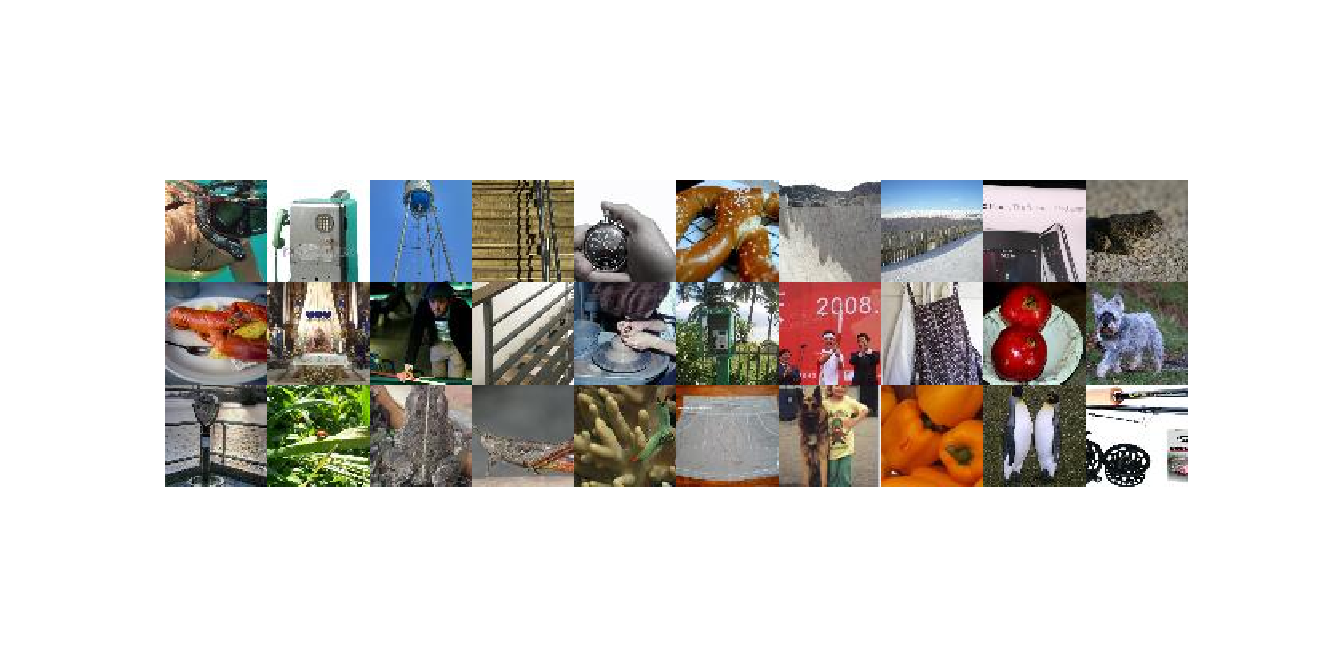
\includegraphics[width=\linewidth]{../images/samples.png}
  \caption[]
  {\small
    30 Samples from the Tiny ImageNet dataset.
  }
  \label{fig:30_samples}
\end{figure}


\iffalse
\subsection{Data Augmentation}
\label{DataAugmentation}
An additional feature that was later added in order to improve the accuracy of the network was data augmentation. Data augmentation was applied batch by batch for each batch used in the training process. The methods of augmentation were the following:

\begin{itemize}
  \item \textbf{Whitening (ZCA):} Applying whitening, may strengthen structure of objects in image by removing redundant information.
  \item \textbf{Horizontal flip:} New perspective on images naturally expands the training data. Vertical flip is available too but in many of the classes an upside-down representation has low resemblance to the image class.
  \item \textbf{Shift:} Shifting images horizontally and vertically allows images to appear in different regions of input space which allows for better generalization.
  \item \textbf{Rotation:} Rotating the images by up to 60 degrees.
\end{itemize}
\fi

\subsection{CNN implementation}

We chose to experiment with different variations of the VGGNet architecture due to its simple implementation and the availability of hardware from the Google Cloud Computing services obtained by KTH for the DD2424 course.

\subsubsection{Implementation specifics}

The network was written and implemented in Python 3.5.2, using the Keras Framework which runs on top of Tensorflow. Numpy was used for data management and Matplotlib to create the graphs. To assist in training and evaluating the networks, we used Google Cloud services for computation power. The specifications of the hardware used was:

\begin{itemize}
  \item 1 x NVIDIA Tesla K80
  \item An unspecified dual core CPU (Unknown CPU Platform on the Google Cloud Platform).
  \item 32 GB RAM memory
  \item 40 GB Disk space.
\end{itemize}

\subsection{Normalization}
Normalization of the input data occurs as two different methods: At first, some models are trained with data where the color channels are divided by the maximum output of the RGB color palettes (255), resulting in the the colors being represented as numbers in ${\rm I\!R} \in [0,1]$.
This was later changed to using Batch Normalization instead for the later training iterations.

\subsection{Evaluating architectures}

The basis of the CNN architecture is inspired by \cite{NIPS2012_4824}, it is summarized in figure \ref{fig:architecture}. However, the network by \cite{NIPS2012_4824} was implemented on the full sized ImageNet dataset. Inspired by architectures mentioned in Previous work \ref{sec:PreviousWork}, we decided to test four configurations, summarized in table \ref{table:3_configurations}.

\begin{figure}[htbp]
  \centering
  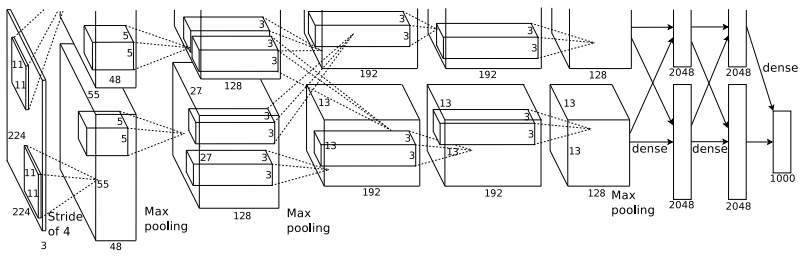
\includegraphics[width=\linewidth]{../images/architecture.jpg}
  \caption[]
  {\small
    Overview of network architecture presented by \cite{NIPS2012_4824}.
  }
  \label{fig:architecture}
\end{figure}

\FloatBarrier
\medskip
\begin{table}[htbp]
\begin{center}
\begin{tabular}{|c|c|c|}

  \hline
  \multicolumn{3}{|c|}{ConvNet Configuration} \\
  \hline

  A & B & C
  \\\hline

  X weight layers & Y weight layers & Z weight layers
  \\\hhline{|=|=|=|}

  \multicolumn{3}{|c|}{input ($64\times64\;RGB\;image$)}
  \\\hline

  conv3-64 & conv3-64 & conv3-64
  \\\hline

  \end{tabular}
\caption[]
{\small
  Configuration of the three different CNNs tested initially. They are inspired from (A) reference, (B) reference and (C) reference.
}
\label{table:3_configurations}
\end{center}
\end{table}


Training was done on the entire Tiny ImageNet dataset, containing 100 000 images and their respective labels. The composition of the dataset is 200 classes with 500 images each. The training data is shuffled before the training process begins. For evaluation, the entire validation dataset was used, containing 10000 images.

\iffalse
Some of the later iterations of training also included data augmentation methods listed in section \ref{DataAugmentation}.The results of each architecture is presented in the Results \ref{sec:Results}.
\fi

\section{Results}
\label{sec:Results}

\subsection{First training iteration: Declaring war on overfitting}

Running over all 4 models presented in table \ref{table:3_configurations} the training and validation loss proved immense after around 5-10 epochs. See figure \ref{fig:4_losses}. We then realized that most of the architectures lacked any form of regularization, except the ones with dropout. That is, without regularization these results are to be expected.

\begin{figure*}
        \centering
        \begin{subfigure}[b]{0.475\textwidth}
            \centering
            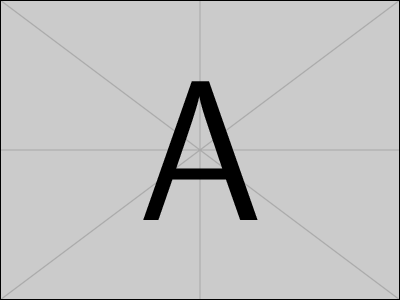
\includegraphics[width=\textwidth]{../images/example-image-a.png}
            \caption[Network2]%
            {{\small Network 1}}
        \end{subfigure}
        \hfill
        \begin{subfigure}[b]{0.475\textwidth}
            \centering
            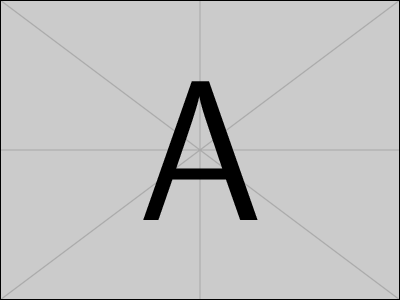
\includegraphics[width=\textwidth]{../images/example-image-a.png}
            \caption[]%
            {{\small Network 2}}
        \end{subfigure}
        \vskip\baselineskip
        \begin{subfigure}[b]{0.475\textwidth}
            \centering
            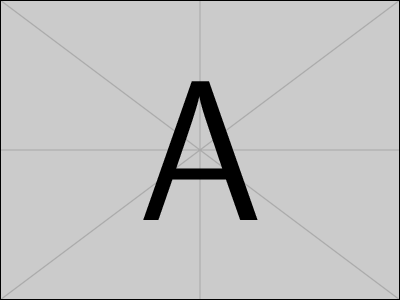
\includegraphics[width=\textwidth]{../images/example-image-a.png}
            \caption[]%
            {{\small Network 3}}
        \end{subfigure}
        \quad
        \begin{subfigure}[b]{0.475\textwidth}
            \centering
            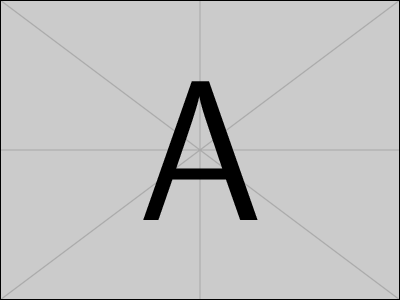
\includegraphics[width=\textwidth]{../images/example-image-a.png}
            \caption[]%
            {{\small Network 4}}
        \end{subfigure}
        \caption[ The average and standard deviation of critical parameters ]
        {\small Caption}
        \label{fig:4_losses}
    \end{figure*}


To combat the overfitting we began tinkering with the different methods we had in our toolbox by testing different combinations of:

\begin{itemize}

  \item L2 regularization
  \item Decay rate
  \item Dropout
  \item Batch normalization

\end{itemize}

%------------------------------------------
\begin{wrapfigure}{r}{0.4\linewidth}
  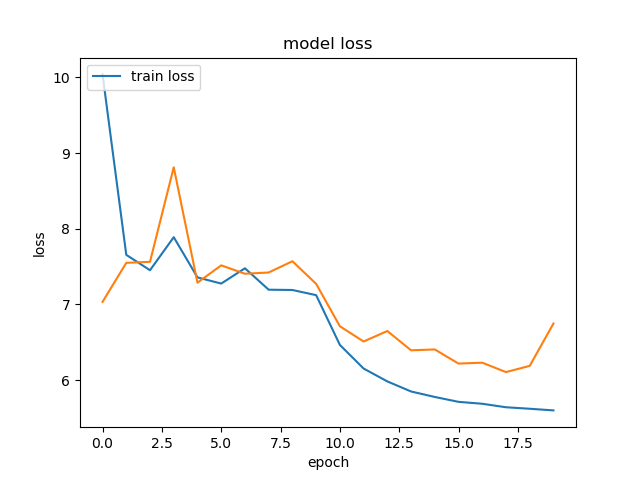
\includegraphics[width=\linewidth]{../images/improved_loss_1.png}
  \caption[]
  {\small Slightly improved convergence of loss functions(not overfitting to the training data) while tinkering with regularization, but significantly increased loss value.}
  \label{fig:loss_improved_1}
\end{wrapfigure}
%------------------------------------------
\FloatBarrier

We also added some additional preprocessing to the dataset by subtracting the mean value of the dataset, feature-wise.

Manually tuning these parameters we found some minor improvements, which is displayed in figure \ref{fig:loss_improved_1}. In this version, we took model D from table \ref{table:3_configurations} and added an $L_{2}$ regularization term of $1e^{-3}$ after each convolutional and fully connected layer, and also increased the number of fully connected layers to 3. In these fully connected layers we increased the dropout to 70\%.


The new model showed a slight improved convergence of the validation loss, but showed an atrocious learning capability due to the high loss values, and thus we found that adding batch normalization, dropout in addition to $L_{2}$ regularization caused the network to shift over to the other side of the spectrum, where instead of overfitting, it had problems learning things. We decided to remove dropout that occurs after the fully connected layers, and instead rely on the $L_{2}$ regularization and add a decay to the learning rate of the network. The decay rate was set to $1e^{-6}$. The Adam solver was initialized with a learning rate of $1e^{-2}$, and we now let it train for longer, 60 epochs in total.

\subsection{Final results}

\begin{figure*}
        \centering
        \begin{subfigure}[b]{0.32\textwidth}
            \centering
            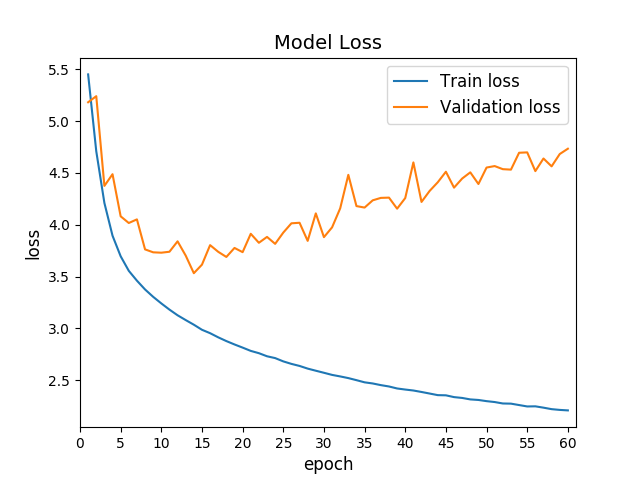
\includegraphics[width=\textwidth]{../images/final_loss.png}
            \caption[]%
            {{\small }}
        \end{subfigure}
        \hfill
        \begin{subfigure}[b]{0.32\textwidth}
            \centering
            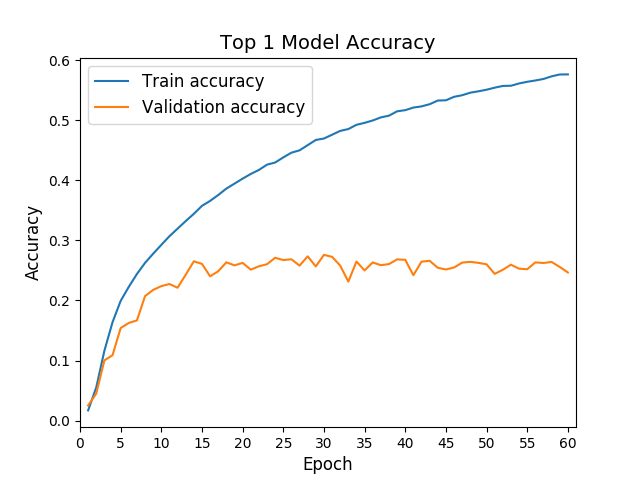
\includegraphics[width=\textwidth]{../images/final_top1.png}
            \caption[]%
            {{\small }}
        \end{subfigure}
        \hfill
        \begin{subfigure}[b]{0.32\textwidth}
            \centering
            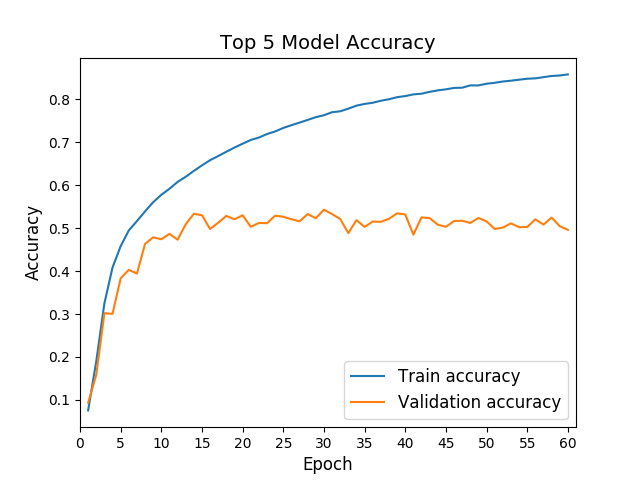
\includegraphics[width=\textwidth]{../images/final_top5.png}
            \caption[]%
            {{\small }}
        \end{subfigure}
        \caption[]
        {\small Training and validation loss of 60 first epochs from best performing model, specified in \ref{table:final_config}. (a) Training and validation loss. (b) Training and validation top-1 accuracy. (c) Training and validation top-5 accuracy.}
        \label{fig:final_plots}
    \end{figure*}


\clearpage
%------------------------------------------
\begin{wraptable}{l}{0.4\linewidth}
  \begin{tabular}{|c|}
  \hline
  \multicolumn{1}{|c|}{ConvNet Config.}
  \\\hline
  Adam, HEI, BN
  \\\hhline{|=|}

  \multicolumn{1}{|c|}{input ($64\times64\times3\;RGB\;image$)}
  \\\hline

  conv-32, 2x2, ReLu, BN
  \\
  conv-32, 2x1, ReLu, BN
  \\
  conv-32, 1x2, ReLu, BN, L2
  \\\hline
  MaxPooling, 2x2
  \\\hline
  conv-48, 2x2, ReLu, BN
  \\
  conv-48, 2x2, ReLu, BN
  \\
  conv-48, 2x2, ReLu, BN, L2
  \\\hline
  MaxPooling, 2x2
  \\\hline
  conv-80, 2x2, ReLu, BN
  \\
  conv-80, 2x2, ReLu, BN
  \\
  conv-80, 2x2, ReLu, BN, L2
  \\\hline
  MaxPooling, 2x2
  \\\hline
  FC-4096, ReLu, BN, L2
  \\\hline
  FC-4096, ReLu, BN, L2
  \\\hline
  FC-4096, ReLu, BN, L2
  \\\hline
  FC-200, SoftMax
  \\\hline
  \end{tabular}
\caption[]
{\small
  Configuration of our final CNN architecture.
}
\label{table:final_config}

\end{wraptable}
%------------------------------------------
The final results found was achieved with a model that has the structure presented in table \ref{table:final_config}. We found additional connected layers in the end combined with L2 regularization helped prevent overfitting to some extent. During our testing it proved a steady learning the 20 first epochs, then it stagnates and begin to overfit. Ideally if we had more time another run with more stricter regularization hopefully would prove more consistent in learning.

The top-1 validation accuracy was 25\% and top-5 validation accuracy 50\%. Plot \ref{fig:final_plots} (a) represents training and validation loss, even though there are fluctuations the validation loss initially follows the training loss nicely, the expanding gap in the higher epochs may as mentioned be countered by increasing regularization. Plot \ref{fig:final_plots} (b) illustrates the evolution of accuracy which, in conjunction with the loss, converges towards the maximal accuracy found.

Summing up all tested models during the experiments, the results of the these models can be found in table \ref{table:accuracy} presented with top-1 accuracy and top-5 accuracy. It's noteworthy that our last model performed worse than the earlier in terms of accuracy. However, we reason that the last model (E) manifested a more consistent behavior during many epochs of training. That is, if model (D) had been trained further is would faster overfit to the training data and generate a non generalizable network. Model (E) on the other hand manifests consistent learning for a longer duration implying minor tweaking of learning parameters may produce a more optimal network. \\



\begin{table}[htbp]
\begin{center}
\begin{tabular}{|l|l|l|l|}
\hline
\textbf{Model} & \textbf{Top-1 val} & \textbf{Top-5 val}  \\
\hline
          A: SGD, RUI                &   17\%  		  &  37\% \\
          B: Adam, RUI, BN           &   22\%  		  &  45\% \\
          C: Adam, RUI, Dropout      &   6\%      	&  20\% \\
          D: Adam, HEI, Dropout, BN  &   29\%  	    &  55\% \\
          E: Adam, HEI, BN, L2       &   25\%       &  50\% \\
          F: Adam, HEI, BN, L2       &   26\%       &  51\% \\

\hline
\end{tabular}
\caption[]
{\small
Accuracy of models.
}
\label{table:accuracy}
\end{center}
\end{table}


% --- Insert accuracy and loss plots here ---

\clearpage
\section{Discussion}
\label{sec:Discussion}

\subsection{Evaluation of method}

There are several flaws in our method and if we where to recreate the experiment we would use a different base architecture for the network.
As seen in figure \ref{wrap-fig:graph_cnns} it is clear that using an VGG structure is not optimal in regard to accuracy, operations and amount of parameters.
A residual network structure seems have the highest potential today with regard to accuracy and operation.
We would probably start with a basic ResNet structure instead of the VGG-net if we were to redo the experiments.
The reason for using a VGG- net was foremost it's easy interpretation and simple implementation. However, the struggle to get an high accuracy due to slow training rate most likely slowed down the process more then the time required to implement and interpret the ResNet structure.
With ResNet in place fewer computations would mean more time on our hands to search for optimal parameters.

Ignoring all gray-scale images in training could have an slight impact on our test accuracy. If we were to recreate the method we would try to figure out an optimal way of handling both grayscale images and RGB images in the same method. One approach would be to reduce all images with 3 channels to grayscale images and create a model optimal for only 1 channel images. Another approach would be to use a assemble methodology with one network adapted for grayscale images and one for RGB images. The lack of classification of the grayscale images also resulted in inability to send our predictions for testing which is made externally by providers of ImageNet.

\subsection{Evaluation of results}

Looking at our result we can see that overfitting is an major issue for our network.
All figures in \ref{fig:architecture} show that the validation loss increases in the final epochs of the models which clearly indicates overfitting.
To combat this issue more regularization was added in the model and the adaption shows results of less overfitting seen in figure \ref{fig:final_plots}.
From table \ref{table:accuracy} it is clear that adding regularization and thus increasing the complexity also increased the models validation accuracy.

If we would continue the implementations the next step would be to add dropout to model E and balance these parameters, maybe by broadly searching a parameter space then progressing to more fine coarse searches, to find optimal parameters of this model.

% As mentioned in the previous section the test accuracy would perhaps have been slightly higher if we would have regarded the fact that some images are in gray-scale.
% Around 2\% of the test images and validation images are gray-scale and we assume that the percentage of gray-scale images is the same in the test data.
% This implies an 2\% loss in accuracy on the test data.

\subsection{Tiny ImageNet State of the art}

In \cite{BarnesStanford} it was showed that using a ResNet18 with data augmentation, dropout and Snapshot Ensembleling they could receive an accuracy of top-5 validation of 81.4\%, top-1 validation of 60.2\% and top-1 test of 53.6\%. This shows with a quite simple network, i.e. not so deep, high accuracy can be achieved when utilizing suitable parameters.

\cite{vCheung} achieve an accuracy of approximately 65\% top-1 error rate on the validation set and an error on the test set of 25.6\%. As of June 12th, 2017 their result was first on the leaderboard for TinyImagenet. They used an ensemble of three models: ResNet101, ResNet152 and DenseNet121. They apply normalization, marginalization and MAP inference in the ensemble architecture.

Our results definitely comes up short comparing against these. A difference lies in number of epochs, we ran 60 which is less than number of epochs used by the implementations mentioned above. But ultimately, the fact our parameters are suboptimal results in our network being prone to overfitting and returns a network that becomes overtrained and generalizes poorly to validation data.

\section{Conclusion}
Making neural networks is a form of art. With so many architectures to choose from the real craftsmanship lies in tuning and tweaking the network accordingly to work properly. We're satisfied with the project as we've learned a lot about CNNs, even though we were hoping to achieve a higher accuracy.


\bibliography{references}{}
\bibliographystyle{plain}

\end{document}
